\documentclass{article}[jsarticle]
\usepackage[T1]{fontenc}
\usepackage[dvipdfmx]{hyperref}
\usepackage{lmodern}
\usepackage{latexsym}
\usepackage{amsfonts}
\usepackage{amssymb}
\usepackage{mathtools}
\usepackage{nccmath}
\usepackage{amsthm}
\usepackage{multirow}
\usepackage[dvipdfmx]{graphicx}
\usepackage{wrapfig}
\usepackage{here}
\usepackage{float}
\usepackage{ascmac}
\usepackage{url}

\title{数理科学概論 課題2}
\author{高林秀 \\ 三宅研究室 博士前期課程1年 \\ V-CampusID : 23vr008n}
\date{\today}

\begin{document}

\maketitle

\setcounter{section}{-1}

\section{問題概要}
本課題の問題は以下1~3の内容である。以降の章でそれぞれについて解答するものとする。

\begin{enumerate}
    \item クロスエントロピーが計算可能であるためには、モデルの出力$\hat{y}$の値はある範囲内でなければならない。
    クロスエントロピーの式からその範囲がどのようになるか、説明せよ。

    \item 以下の表には、5つのデータからなる2値分類問題で、case 1~6 の6つの場合において、モデル出力がまとめられている。
    それぞれのケースについて、5つのデータのクロスエントロピーの平均値を求めよ。\par 
    また、各ケースの二乗平均誤差 (モデル出力と正解ラベルの差の二乗の平均値) も求めよ。
    \begin{figure}[H]
        \centering
        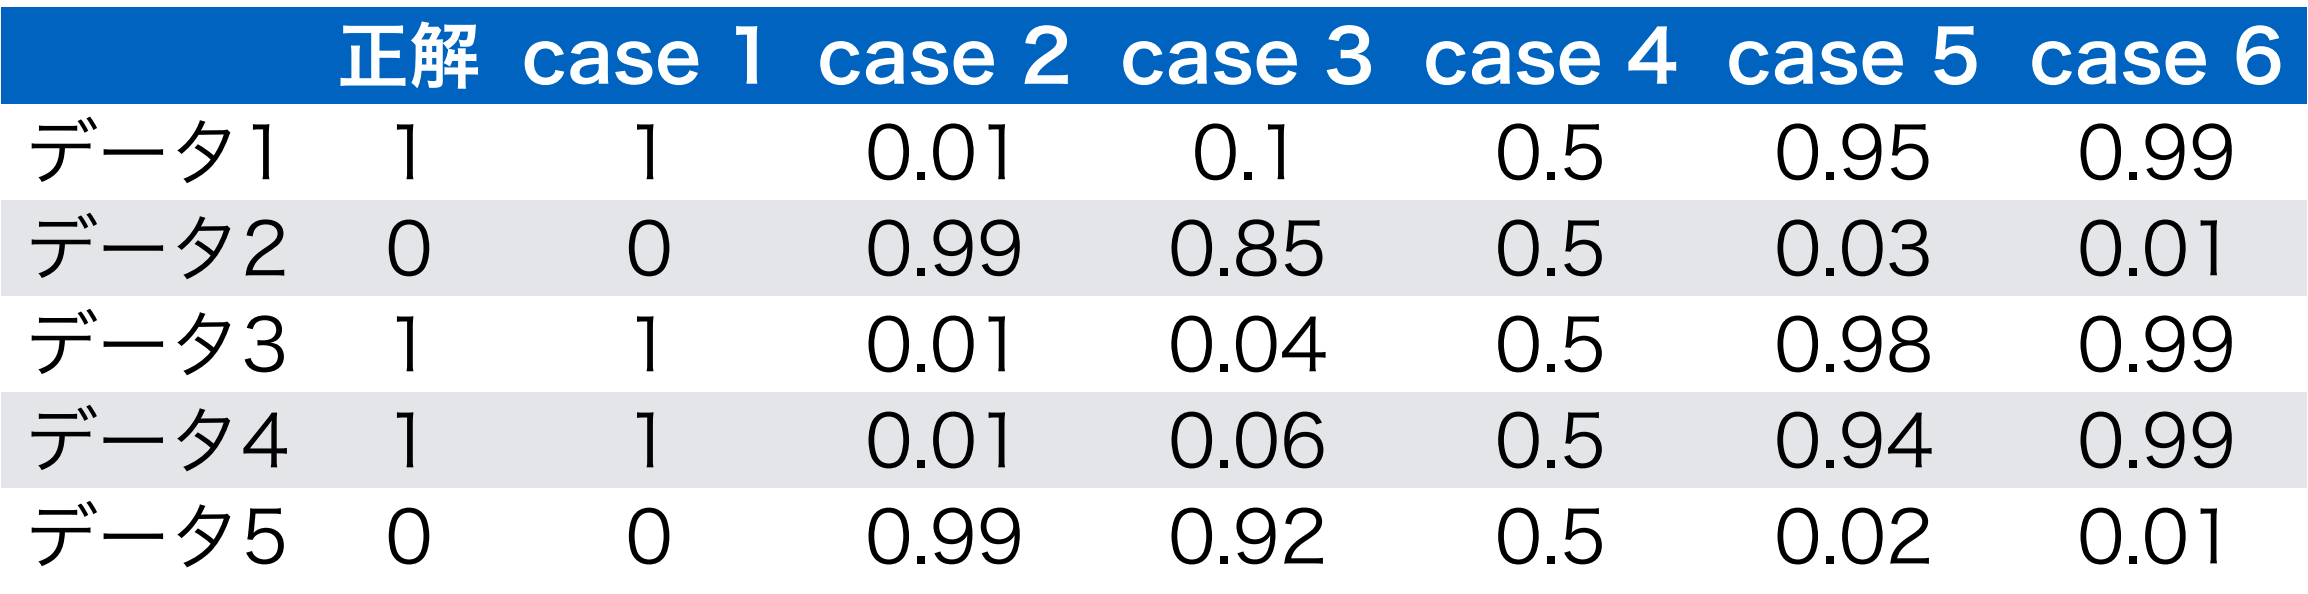
\includegraphics[scale=0.3]{./2023-06-23215207.png}
    \end{figure}

    \item クロスエントロピーと二乗平均誤差について、(2) で計算した値からわかる範囲で共通点と相違点について考察せよ。
    ただし、各ケースでの値を直接比較するのではなく、ケースの変化に対して値がどのように変化していくかについて考察すること。
    
\end{enumerate}

\subsection{制約条件}
この問題で求めるクロスエントロピーは、対数の底を $e$ としたものとすること。$0\log_{e}0$は数学においては本来計算不可能な量だが、
本問題においてもし出てきた場合には0としてよいものとする。


\section{問1} 
\subsection{問題文}
クロスエントロピーが計算可能であるためには、モデルの出力$\hat{y}$の値はある範囲内でなければならない。クロスエントロピーの式からその範囲がどのようになるか、説明せよ。
\subsection{解答}
\section{問2}
\subsection{問題文}
以下の表には、5つのデータからなる2値分類問題で、case 1~6 の6つの場合において、モデル出力がまとめられている。
それぞれのケースについて、5つのデータのクロスエントロピーの平均値を求めよ。\par 
また、各ケースの二乗平均誤差 (モデル出力と正解ラベルの差の二乗の平均値) も求めよ。
\begin{figure}[H]
    \centering
    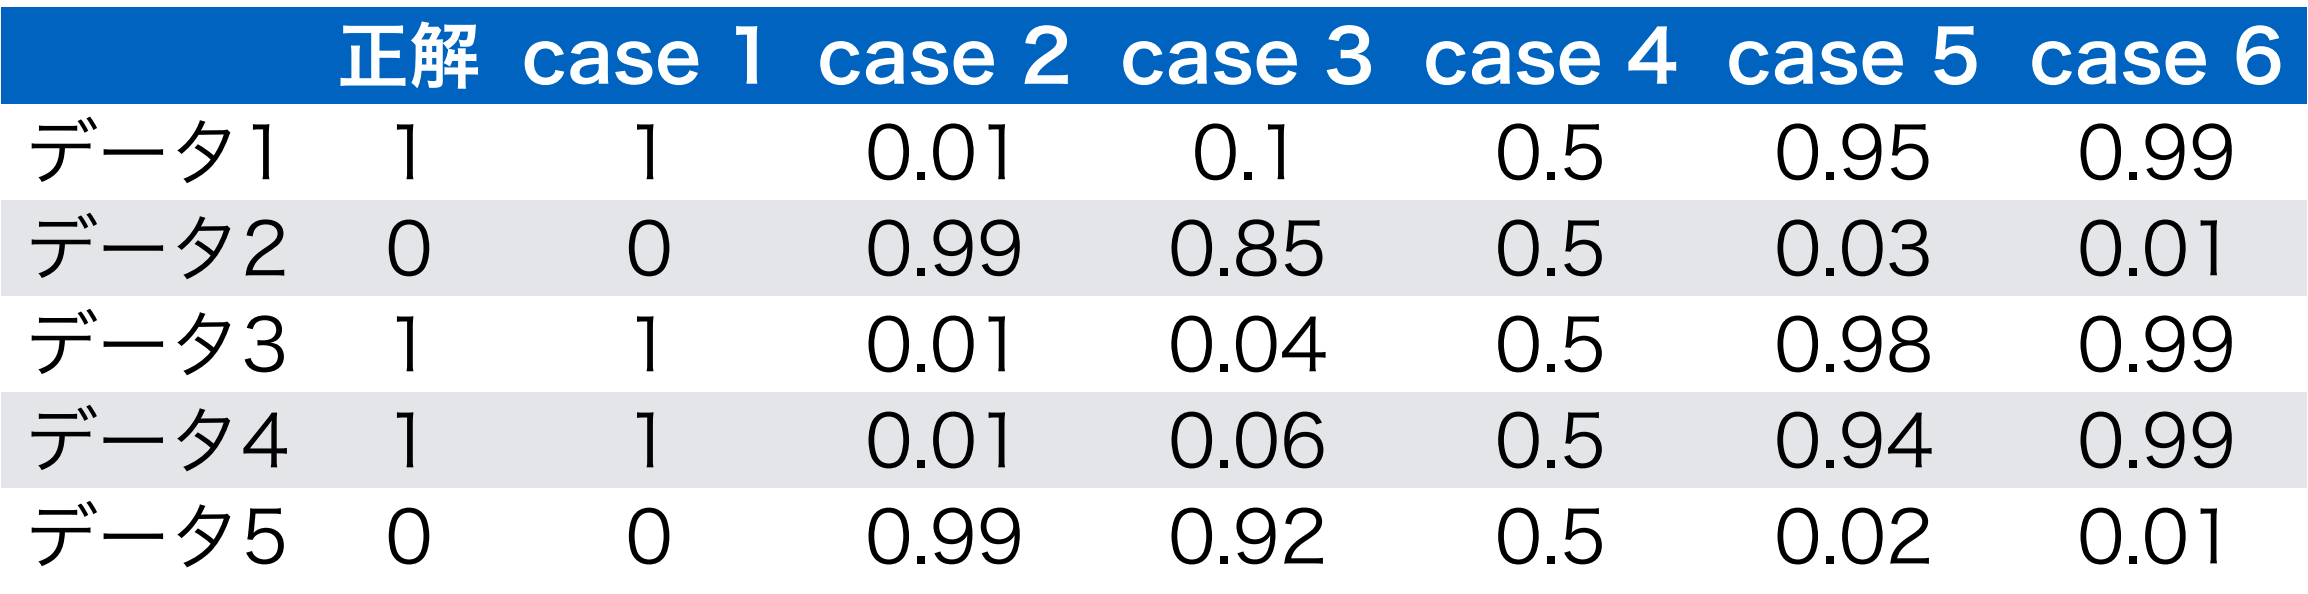
\includegraphics[scale=0.3]{./2023-06-23215207.png}
\end{figure}
\subsection{解答}
\section{問3}
\subsection{問題文}
クロスエントロピーと二乗平均誤差について、(2) で計算した値からわかる範囲で共通点と相違点について考察せよ。
ただし、各ケースでの値を直接比較するのではなく、ケースの変化に対して値がどのように変化していくかについて考察すること。
\subsection{解答}


  

\end{document}